\subsection{The Graph Coloring Game}
\label{sec:2.1}

\begin{flushleft}

    The \emph{Graph Coloring Problem} (GCP) is one of the most well-known problems in graph theory. It involves assigning colors to vertices in a graph such that no two adjacent vertices share the same color, and using the minimum number of colors, also known as the chromatic number \cite{watkins2023generating}.\\~\\

    In this study, we shift our focus from finding the chromatic number across graph configurations to a slightly different approach. Rather than solving the GCP itself, we use the concept of graph coloring to define a dynamic game that allows us to study the evolutionary dynamics in multi-agent interactions. Nonetheless, the concept of the chromatic number will reappear in our analysis, not as a problem to be solved but as a way to color the grid, i.e., a style of play. Through this, we aim to gain insights into whether individuals with this preference actually ensure good collaboration, or if other styles of play are more effective when combined. To provide a consistent framework for our study, we assume a fixed grid configuration and a fixed number of colors available to the agents, as a static base to study agent interactions. Specifically, we set the number of colors to match the total number of blocks in the grid, allowing agents to consider even the worst-case scenario where assigning a unique color to each block is the only valid solution.
    %
    \begin{figure}[h]
        \centering
        \begin{minipage}{0.46\linewidth}
            \centering
            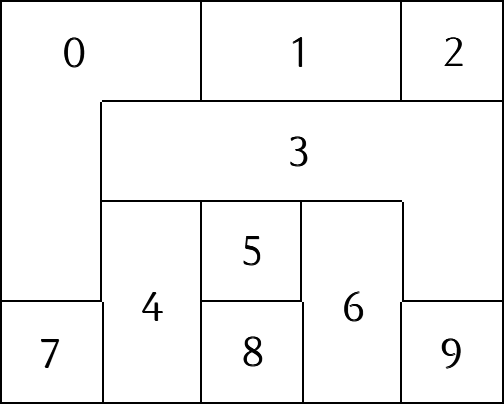
\includegraphics[width=\linewidth]{images/grid.png}
        \end{minipage}
        \hfill
        \begin{minipage}{0.49\linewidth}
            \centering
            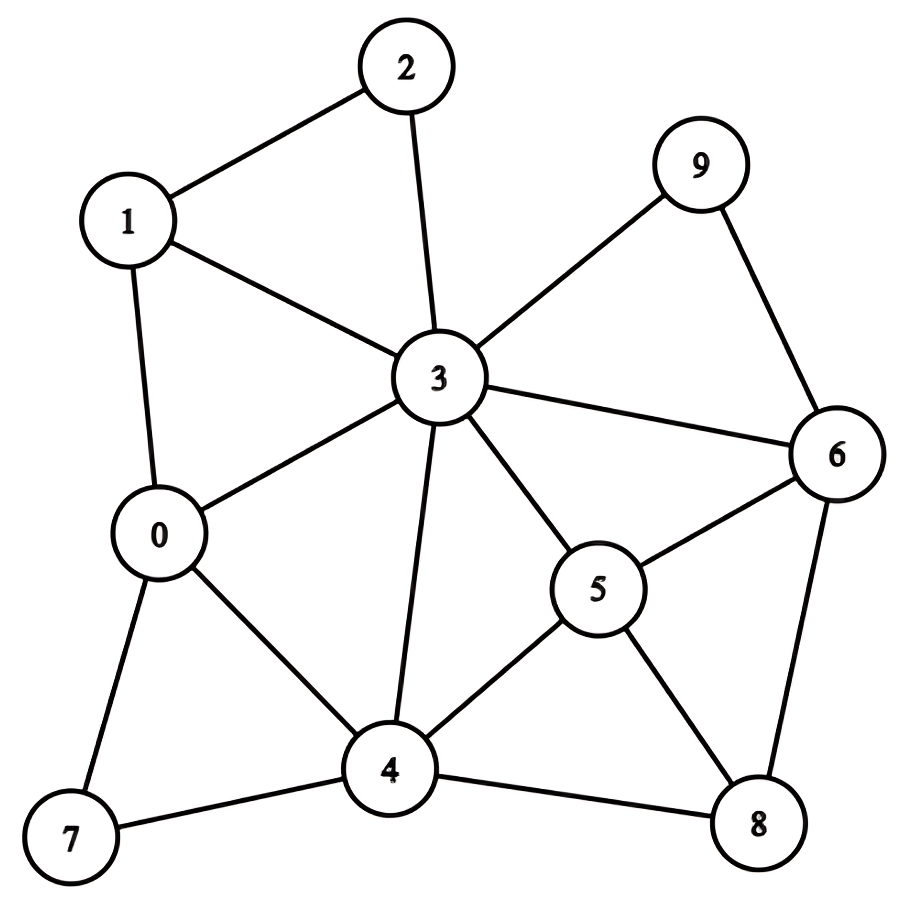
\includegraphics[width=\linewidth]{images/graph.png}
        \end{minipage}
        \caption{A snaphsot of the game environment in grid and graph forms.}
        \label{fig:grid_and_graph}
    \end{figure}
    %

    \subsubsection{State and Action Space}

    \begin{flushleft}

        The graph in the game corresponds to a grid of blocks, where each block is defined as one or more merged cells within the two-dimensional matrix. At the beginning of the game, the grid is initialized with a random number of rows and columns ($n \times m$), and this configuration remains the same throughout the entire game. The environment then randomly combines cells to create blocks. Merging cells is important as it allows for complex neighboring relationships to be defined, expanding beyond the standard constraints between adjacent blocks. In our experimental setup we assume a $4 \times 5$ grid with 10 blocks as illustrated in Figure~\ref{fig:grid_and_graph}.\\~\\

        Blocks can be either (a) colored by the agents, (b) white (free to be colored) or (c) hidden (their colors cannot be observed and they can not be re-colored by the agents). Initially all blocks in the grid are white and hidden. These hidden blocks are symbolically represented in gray. Let $G$ denote the grid environment, $B$ the set of blocks in that environment and $CR$ the set of possible colors that an agent can use for coloring blocks. Then our first assumption is that every block $b$ in $B$ can potentially be assigned any color $c$ from $CR$:
        %
        \begin{equation}
            \forall b \in B, \, \forall c \in CR, \, (b, c) \in R 
            \label{eq:bc}
        \end{equation}
        %

        The set of agents' actions $A$ is defined to be the Cartesian product of the set of blocks $B$ and the set of the available colors $CR$, denoted as:
        %
        \begin{equation}
            A = B \times CR = \{(b, c) \mid b \in B, \, c \in CR\} 
            \label{eq:action_space}
        \end{equation}
        %

        To specify states, let $CR^*$ include the elements of $CR$, and two additional elements representing hidden and white blocks: $CR^* = CR \cup \{\text{hidden}, \text{white}\}$. We define state $s$ as the Cartesian product of $B$ and $CR^*$, denoted as:
        %
        \begin{equation}
            s = \{(b_i, c_i), i=1, \dots, |B|\}, s.t. \forall b \in B, \, \exists \text{a unique } c \in CR^*\text{, with } (b,c) \in s
            \label{eq:state}
        \end{equation}
        %

        We consider the Graph Coloring Game (GCG) to be a two-player game that unfolds over multiple rounds. At the beginning of each round, the environment reveals the color of some of the hidden blocks, if any. The number of blocks that get un-hidden is random, which implies that the state of the graph is influenced not only by the agents' actions. We therefore consider the game to be stochastic. After the state update from the environment, the agents simultaneously choose their actions. As soon as all blocks in $B$ are uncovered and colored, the game ends.
    
    \end{flushleft}

    \subsubsection{Reward Function}

    \begin{flushleft}

        The reward function in the GCG is designed to encourage agents to adopt effective strategies for coloring blocks while discouraging undesirable actions. The total reward that an agent receives during the game is the sum of multiple components, including gains, penalties, sanctions, delays and adopted preferences.\\~\\

        It is defined as follows:

        \begin{enumerate}
            \item \textbf{Gains:} An agent receives a gain of +1 for each neighboring block of $b$ that has a different color than the chosen color $c$. This reward encourages agents to color neighboring blocks with different colors, in line with the rules of the GCP, where adjacent blocks must have distinct colors.
            
            \item \textbf{Penalties:} An agent receives a penalty of -2 for each neighboring block that shares the same color $c$ as the chosen one. This reward serves the same purpose of ensuring proper coloring by discouraging agents from coloring adjacent blocks with the same color, which would violate the rules of the GCP.
            
            \item \textbf{Sanctions:} An agent receives a sanction, a large negative reward of -10, when it attempts to color a hidden block or a block that has already been colored. This reward ensures that agents follow the game’s rules and do not waste their actions on illegal moves.
            
            \item \textbf{Delays:} If both agents attempt to color the same block $b$ during the same round, a small negative reward of -1 is applied to both agents. This reward represents the time spent in resolving the conflict between the two agents over who will color the block.
            
            \item \textbf{Preference-Adoption:} Regardless of whether an agent’s action is successful, unsuccessful, or forbidden, the agent receives a preference-adoption reward for adhering to specific preferences or styles of play. This reward encourages agents to adopt behaviors that align with desired goals.
        \end{enumerate}

    \end{flushleft}

\end{flushleft}